% AWS Lab_2.tex - AWS Lab 2 for Cloud Computing class (Spring 2015)
% Chanmann Lim - March 2015

\documentclass[a4paper]{article}

\usepackage[margin=1 in]{geometry}
\usepackage{listings}
\usepackage{graphicx}
\usepackage{float}

\begin{document}
\title{CS 7001-03: Report for AWS Lab 2 - AWS Resource Discovery and Instance Setup}
\author{Chanmann Lim\\ 
	\texttt{cl9p8@mail.mail.missouri.edu}}
\date{March 03, 2015}
\maketitle


Install \texttt{awscli} tool via easy\_install \texttt{pip} on Mac OS.

% ---------------------------------------- 1 ----------------------------------------
\paragraph{1. } Create an AWS key pair using \texttt{ec2 create-key-pair} command with \texttt{--key-name} option set to 'cloud-key':
\begin{verbatim}
# aws ec2 create-key-pair --key-name cloud-key
\end{verbatim}

Delete a key pair using \texttt{ec2 delete-key-pair} command with \texttt{--key-name} option set to 'cloud-key':
\begin{verbatim}
# aws ec2 delete-key-pair --key-name cloud-key
\end{verbatim}

% ---------------------------------------- 2 ----------------------------------------
\paragraph{2. } Create a security group in AWS. \\

Use \texttt{ec2 create-security-group} command with options
\begin{description}
\leftskip 0.4in
\parindent -0.4in
	\item[\texttt{--group-name} : ] set security group name.
	\item[\texttt{--description} : ] set security group description.
\end{description}

and adding inbound traffic rule to security group via \texttt{ec2 authorize-security-group-ingress} command with options
\begin{description}
\leftskip 0.4in
\parindent -0.4in
	\item[\texttt{--group-name} : ] set security group name.
	\item[\texttt{--protocol} : ] set IP protocol eg. tcp, udp or icmp.
	\item[\texttt{--port} : ] set tcp or tcp port range.
	\item[\texttt{-cidr} : ] set IP range.
\end{description}
\begin{verbatim}
# aws ec2 create-security-group  \
      --group-name cloud-group   \
      --description "Open ports"
# aws ec2 authorize-security-group-ingress \
      --group-name cloud-group             \
      --protocol tcp                       \
      --port 22                            \
      --cidr 0.0.0.0/0
# aws ec2 authorize-security-group-ingress \
      --group-name cloud-group             \
      --protocol tcp                       \
      --port 22                            \
      --cidr 0.0.0.0/0
# aws ec2 authorize-security-group-ingress \
      --group-name cloud-group             \
      --protocol tcp                       \
      --port 22                            \
      --cidr 0.0.0.0/0
\end{verbatim}

Delete security group via \texttt{ec2 delete-security-group} command with \texttt{--group-name} option set to 'cloud-group'.

\begin{verbatim}
# aws ec2 delete-security-group --group-name cloud-group
\end{verbatim}

% ---------------------------------------- 3 ----------------------------------------
\paragraph{3. } Enter the commands below and describe in detail the results; you will need an AMI available. Once the command is executed, using aws-cli commands, terminate the instances, delete ‘cloud-key’ and ‘cloud-group’. Include screenshot. \\
ec2-run-instances ami-xxxxxx --instance-type t1.micro --instance-count 2  --key cloud-key  --group cloud-group  --region us-east-1

% ---------------------------------------- 4 ----------------------------------------
\paragraph{4. } Get status information of all instances using aws-cli commands.
\begin{verbatim}
# aws ec2 describe-instance-status
\end{verbatim}
\begin{figure}[H]
  \centering
    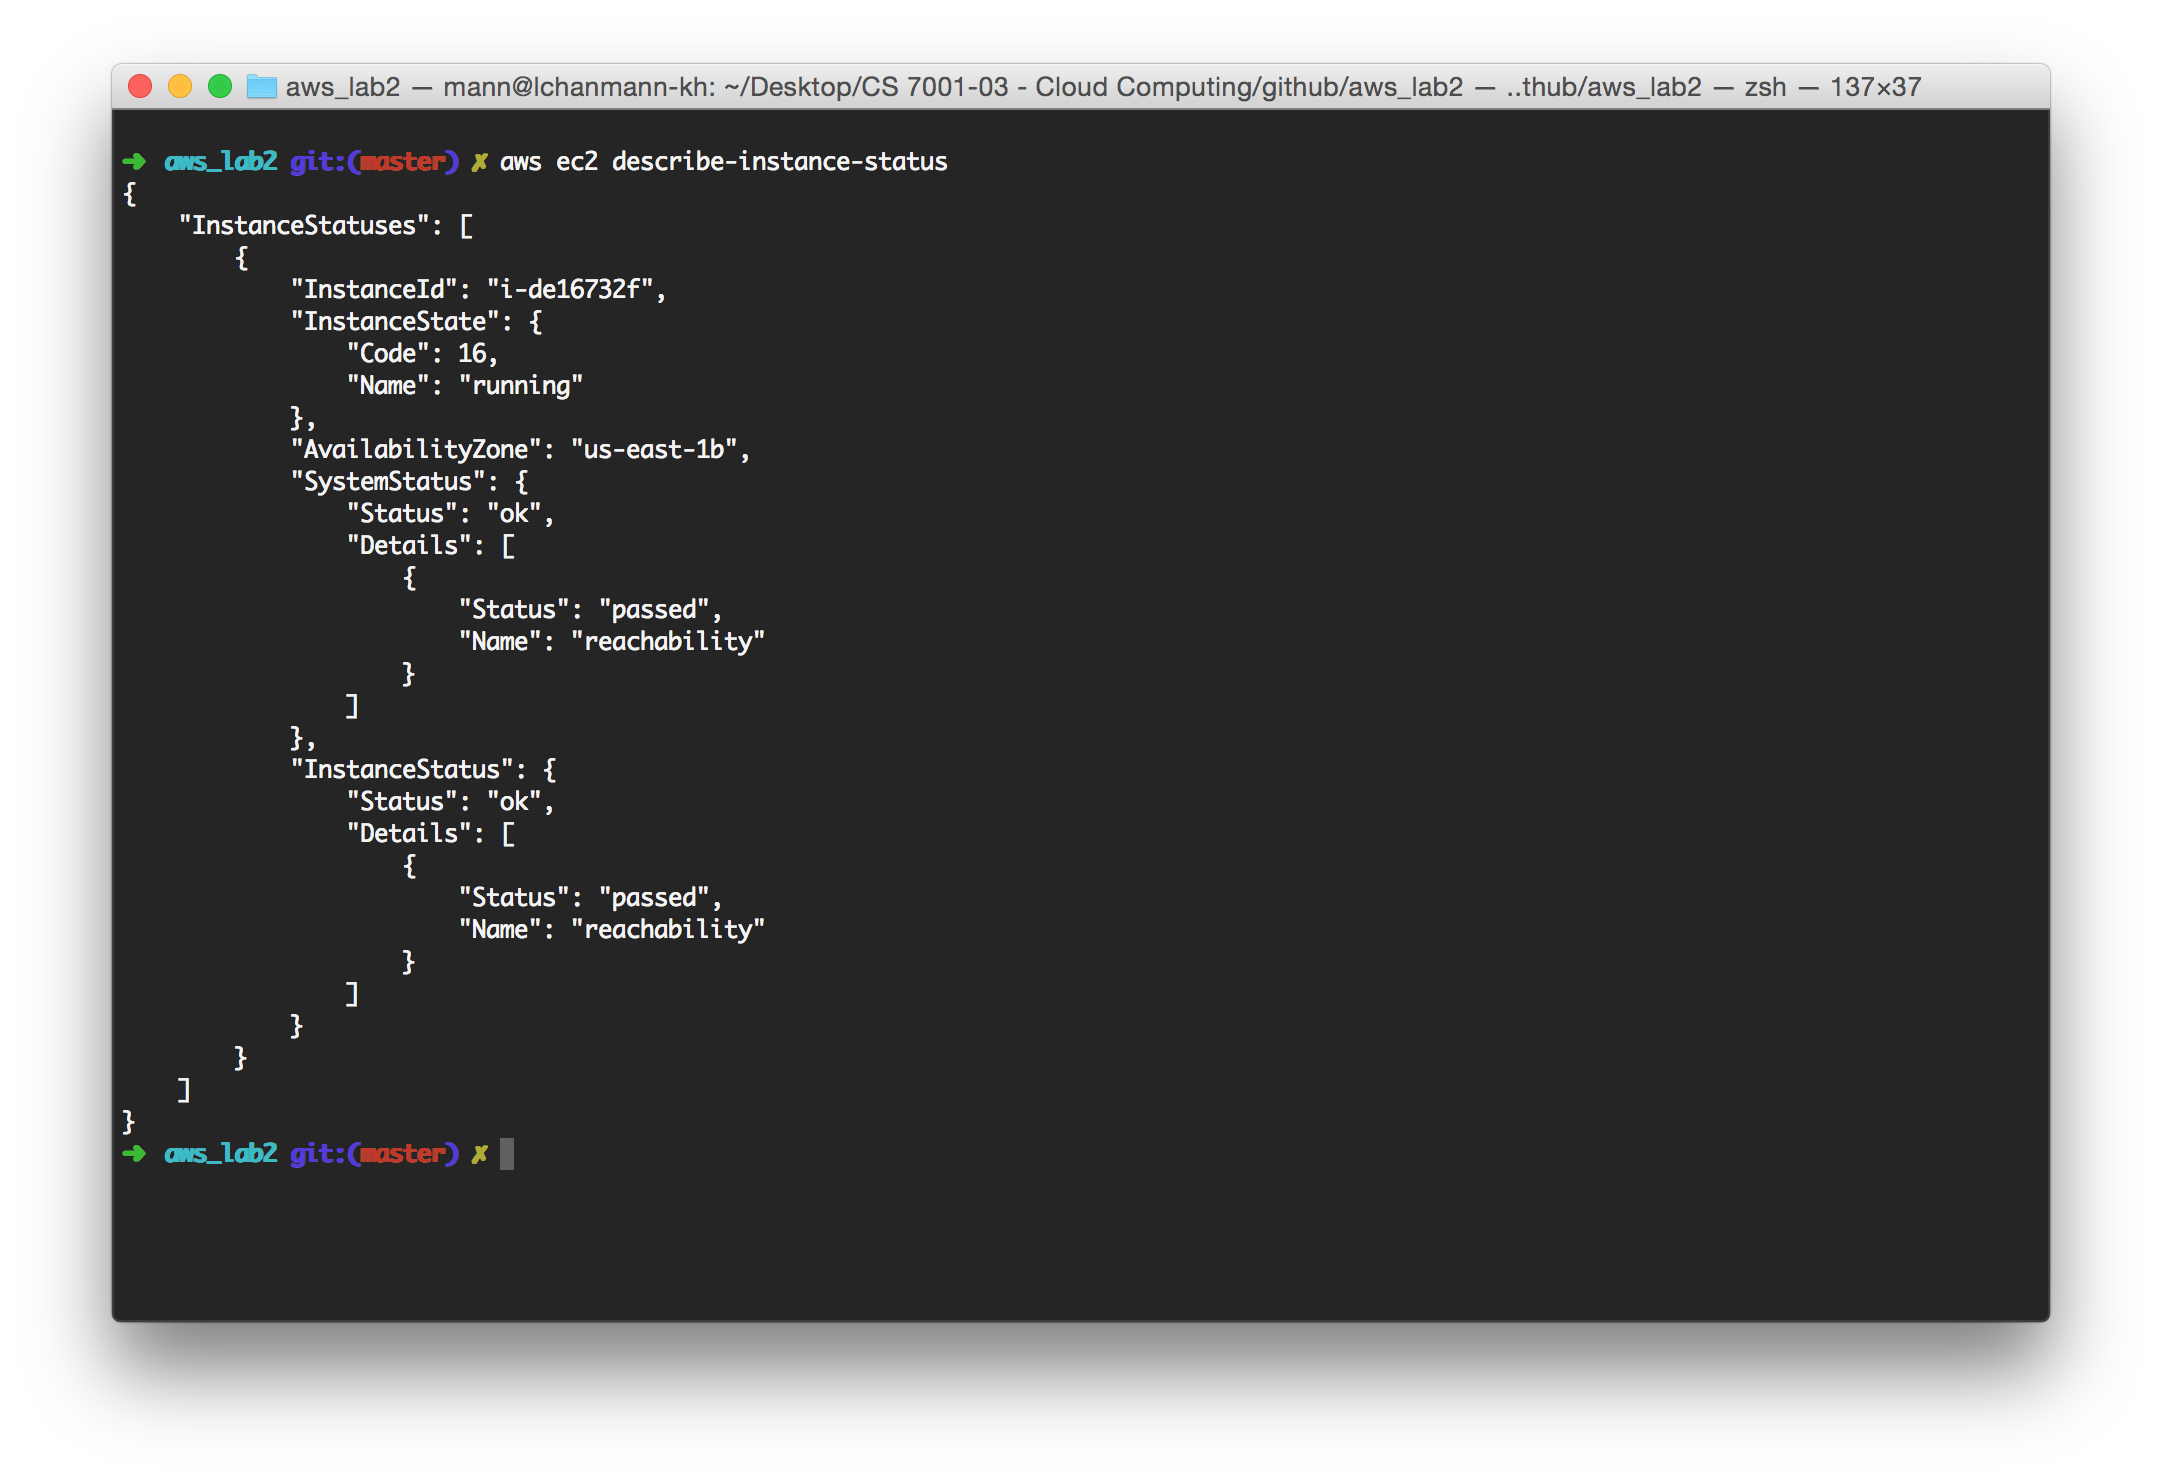
\includegraphics[scale=.4]{instance_status.png}
  \caption{AWS instances status}
\end{figure}

% ---------------------------------------- 5 ----------------------------------------
\paragraph{5. } Create snapshot command: \texttt{ec2 create-snapshot} with options
\begin{description}
\leftskip 0.4in
\parindent -0.4in
	\item[\texttt{--volume-id} : ] set EBS volume to be snapshot.
	\item[\texttt{--description} : ] set snapshot description.
\end{description}
\begin{verbatim}
# aws ec2 create-snapshot      \
      --volume-id vol-54c4644f \
      --description "Backup"
\end{verbatim}

Delete snapshot command: \texttt{ec2 delete-snapshot} with \texttt{--snapshot-id} option.
\begin{verbatim}
# aws ec2 delete-snapshot --snapshot-id snap-51cf8cd0
\end{verbatim}


% ---------------------------------------- 6 ----------------------------------------
\paragraph{6. } Add a new EBS volume with \texttt{ec2 create-volume} with options:
\begin{description}
\leftskip 0.4in
\parindent -0.4in
	\item[\texttt{--size} : ] set volume size (in GB).
	\item[\texttt{--availability-zone} : ] set availability zone of the volume.
\end{description}
\begin{verbatim}
#aws ec2 create-volume --size 3 --availability-zone us-east-1b
\end{verbatim}

Attach the volume to the running instance (i-de16732f) via \texttt{ec2 attach-volume} with options:
\begin{description}
\leftskip 0.4in
\parindent -0.4in
	\item[\texttt{--volume-id} : ] set volume id to attach.
	\item[\texttt{--instance-id} : ] set instance id to be attached to.
	\item[\texttt{--device} : ] set device name with which the instance will use to interact.
\end{description}
\begin{verbatim}
#aws ec2 attach-volume        \
     --volume-id vol-3ae79321 \
     --instance-id i-de16732f \
     --device /dev/sdh
\end{verbatim}
\begin{figure}[H]
  \centering
    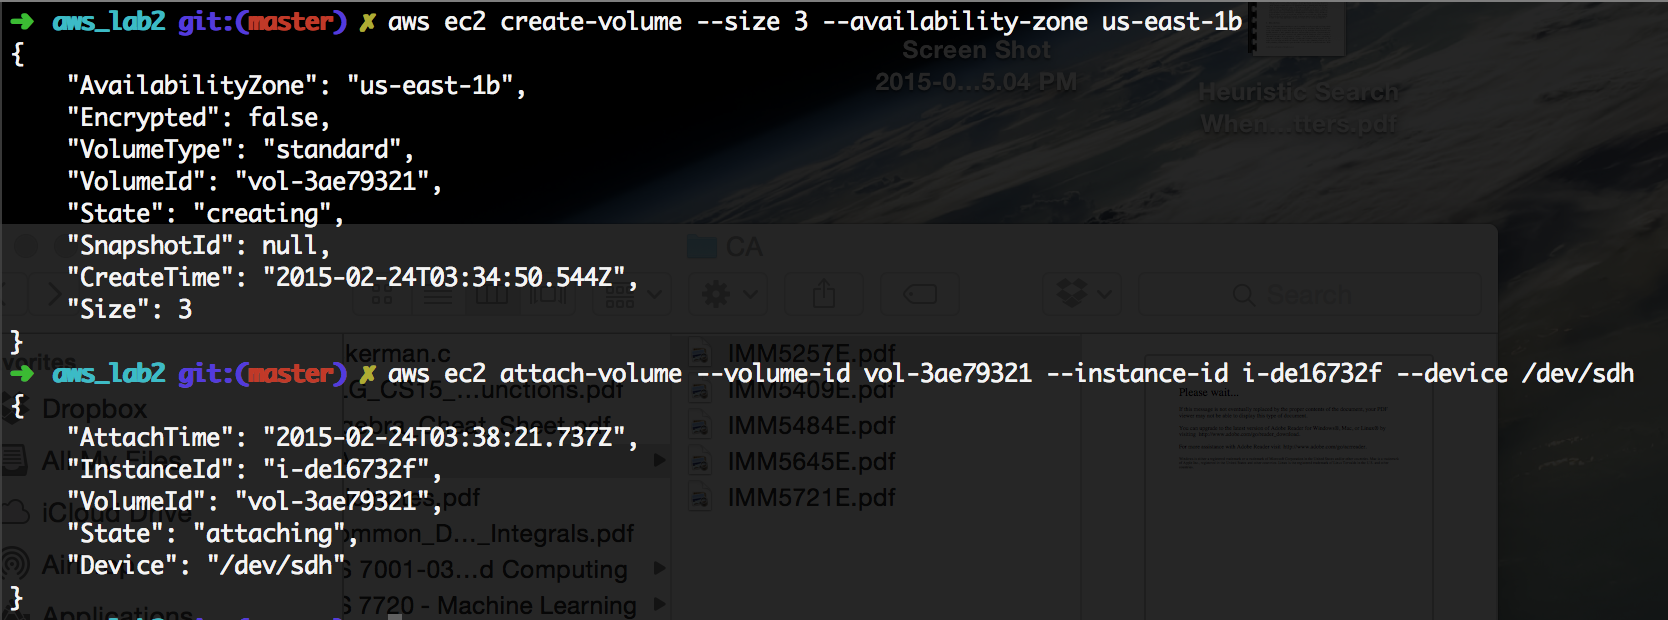
\includegraphics[scale=.4]{attaching_volume.png}
  \caption{Create and attach volume using aws-cli}
\end{figure} 
\begin{figure}[H]
  \centering
    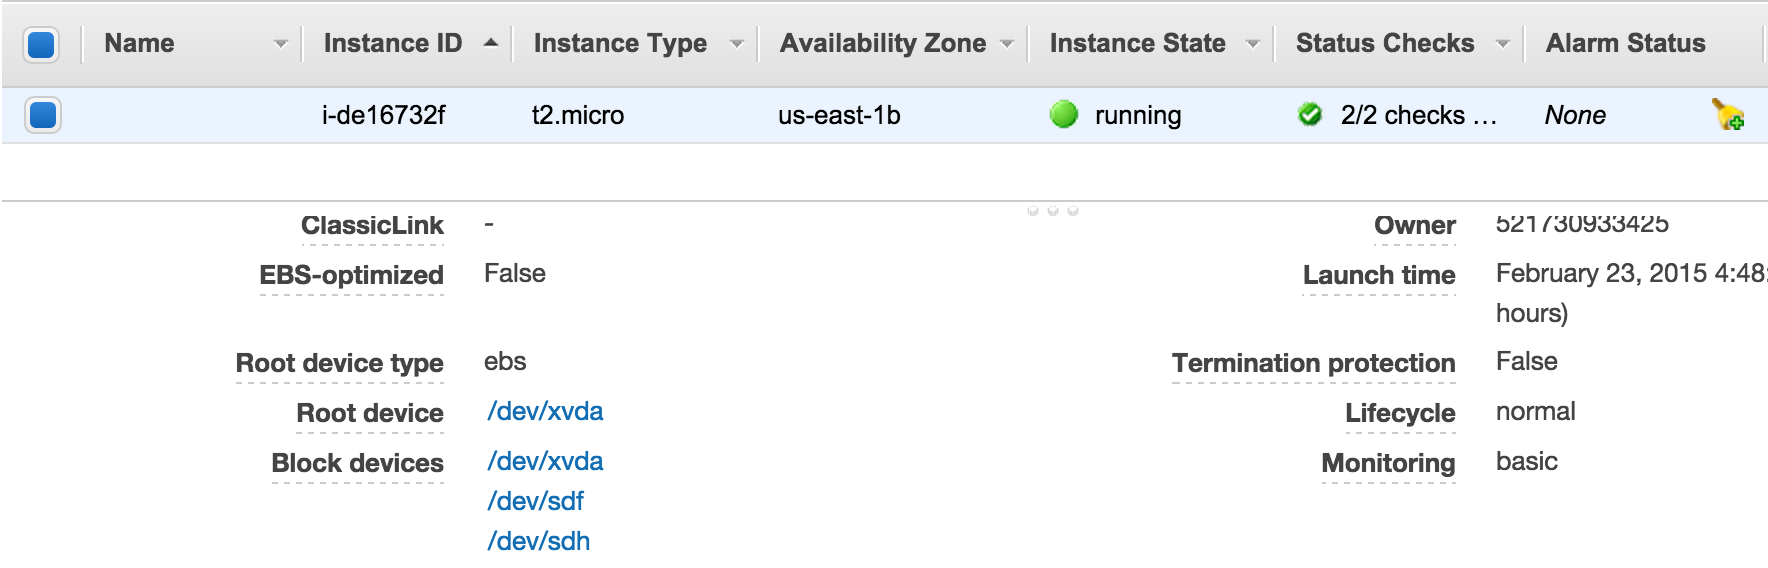
\includegraphics[scale=.4]{attached_volume.png}
  \caption{The new volume is attached to /dev/sdh}
\end{figure} 

% ---------------------------------------- 7 ----------------------------------------
\paragraph{7. } Provide a screenshot taken in Step 3.4.2 \\

\texttt{http://ec2-52-1-133-200.compute-1.amazonaws.com/} \\
\begin{figure}[H]
  \centering
    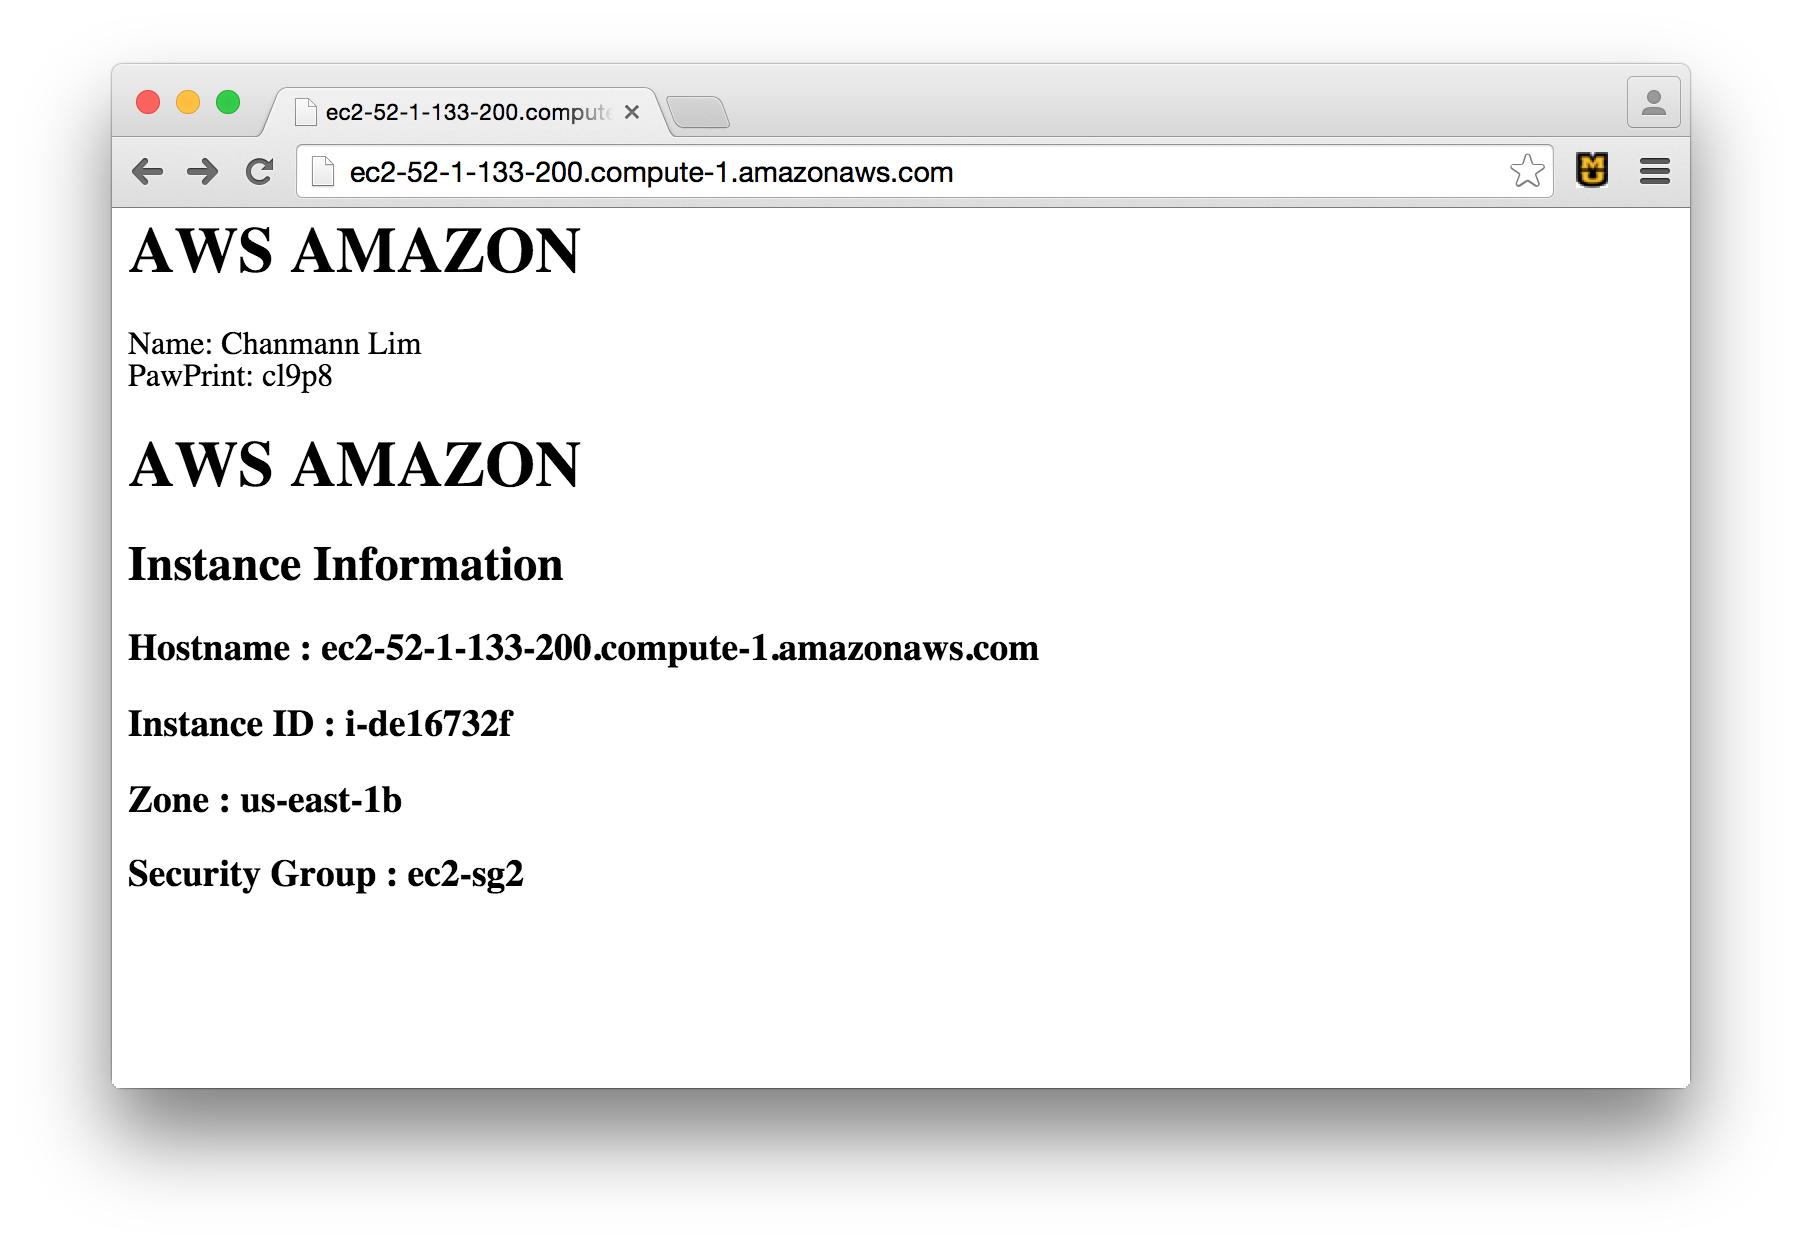
\includegraphics[scale=.4]{aws_web_server.png}
  \caption{AWS web server}
\end{figure} 

% ---------------------------------------- 8 ----------------------------------------
\paragraph{8. } Briefly explain the 6 AWS best practices described by Amazon AWS. 

\end{document}